\documentclass{tufte-handout}

%\geometry{showframe}
%\geometry{showframe}% for debugging purposes -- displays the margins

\usepackage{amsmath}
\usepackage{amssymb}
\usepackage{cleveref}
\usepackage{hyperref}  % Add this after cleveref
\crefname{Proposition}{Proposition}{Propositions}
\Crefname{Proposition}{Proposition}{Propositions}
\crefname{Theorem}{Theorem}{Theorems}
\Crefname{Theorem}{Theorem}{Theorems}
\crefname{Definition}{Definition}{Definitions}
\Crefname{Definition}{Definition}{Definitions}
\crefname{Corollary}{Corollary}{Corollaries}
\Crefname{Corollary}{Corollary}{Corollaries}
\crefname{Lemma}{Lemma}{Lemmas}
\Crefname{Lemma}{Lemma}{Lemmas}
\crefname{Example}{Example}{Examples}
\Crefname{Example}{Example}{Examples}
\crefname{figure}{Figure}{Figures}
\Crefname{figure}{Figure}{Figures}
\usepackage{amsthm}

% Set up the images/graphics package
\usepackage{graphicx}
\setkeys{Gin}{width=\linewidth,totalheight=\textheight,keepaspectratio}
\graphicspath{{graphics/}}

% The following package makes prettier tables.  We're all about the bling!
\usepackage{booktabs}

% The units package provides nice, non-stacked fractions and better spacing
% for units.
\usepackage{units}

% The fancyvrb package lets us customize the formatting of verbatim
% environments.  We use a slightly smaller font.
\usepackage{fancyvrb}
\fvset{fontsize=\normalsize}

% Small sections of multiple columns
\usepackage{multicol}

% Provides paragraphs of dummy text
\usepackage{lipsum}

% Defines colors
\usepackage{xcolor}
\definecolor{blue}{cmyk}{0.63, 0.37, 0, 0.57}     
\definecolor{ltblue}{RGB}{78,150,179}

% These commands are used to pretty-print LaTeX commands
\newcommand{\doccmd}[1]{\texttt{\textbackslash#1}}% command name -- adds backslash automatically
\newcommand{\docopt}[1]{\ensuremath{\langle}\textrm{\textit{#1}}\ensuremath{\rangle}}% optional command argument
\newcommand{\docarg}[1]{\textrm{\textit{#1}}}% (required) command argument
\newenvironment{docspec}{\begin{quote}\noindent}{\end{quote}}% command specification environment
\newcommand{\docenv}[1]{\textsf{#1}}% environment name
\newcommand{\docpkg}[1]{\texttt{#1}}% package name
\newcommand{\doccls}[1]{\texttt{#1}}% document class name
\newcommand{\docclsopt}[1]{\texttt{#1}}% document class option name

% Package for title style
\usepackage{sectsty}
\usepackage[utf8]{inputenc}

% Sets section number style
\setcounter{secnumdepth}{3} % uncomment this, if desired
\renewcommand\thesection{\color{white}\arabic{section}}

% Sets title style
\makeatletter
  \renewcommand{\paragraph}{\@startsection{paragraph}%
    {4}{\z@}{-1ex \@plus -1ex \@minus -.3ex}%
    {0.5ex \@plus .2ex}{\normalfont\normalsize\bfseries}}
\makeatother

\makeatletter
  \renewcommand{\subsection}{\@startsection{subsection}%
    {3}{-1.8em}{-3ex \@plus -1ex \@minus -.2ex}%
    {1.5ex \@plus .2ex}
    {\hspace*{-5.5em}\fcolorbox{ltblue}{ltblue}{\parbox[c][1.0ex][b]{4em}{\phantom{space}}}
    \normalfont\large\itshape\color{ltblue}}}
\makeatother

\makeatletter
  \renewcommand{\section}{\@startsection{section}%
    {3}{-1.01em}{-3ex \@plus -1ex \@minus -.2ex}%
    {1.5ex \@plus .2ex}
    {\hspace*{-5.5em}\fcolorbox{blue}{blue}{\parbox[c][1.0ex][b]{4em}{\phantom{space}}}
    \normalfont\Large\itshape\color{blue}}}
\makeatother

% Sets theorem style
\usepackage{thmtools}
\usepackage{transparent}
\definecolor{theb}{rgb}{0.67, 0.80, 0.91}

\declaretheorem[shaded={bgcolor=Lavender,
    textwidth=30em}]{Definition} % Colorbox-styled Theorem 
\declaretheorem[shaded={bgcolor=Lavender,
    textwidth=30em}]{Theorem} % Colorbox-styled Theorem 
\declaretheorem[shaded={bgcolor=Thistle,
    textwidth=30em}]{Corollary} % Colorbox-styled Theorem
\declaretheorem[shaded={bgcolor=PeachPuff,
    textwidth=30em}]{Proposition} % Colorbox-styled Proposition
\declaretheorem[shaded={bgcolor=Thistle,
    textwidth=30em}]{Lemma} % Colorbox-styled Lemma
\declaretheorem[shaded={rulecolor=Lavender,
    rulewidth=2pt, bgcolor={rgb}{1,1,1}}]{Example-1} % Colorbounded-styled Theorem
\declaretheorem[thmbox=L]{boxtheorem L} % Theorem box L-size
\declaretheorem[thmbox=M]{Example} % Theorem box M-size
\declaretheorem[thmbox=S]{Formula} % Theorem box S-size
\declaretheorem[thmbox=S]{Statement} % Theorem box S-size

% set up pdf bookmark depth
\hypersetup{bookmarksdepth=3}

% In the preamble, add these figure-specific settings
\crefformat{figure}{figure~#2#1#3}
\Crefformat{figure}{Figure~#2#1#3}
\crefrangeformat{figure}{figures~#3#1#4 to~#5#2#6}
\Crefrangeformat{figure}{Figures~#3#1#4 to~#5#2#6}

% ------------------------------------------------------------
\title{NEUR503: Computational Neuroscience}
\author[Matthew He]{Matthew He}
% \date{December 1, 2024}
% if the \date{} command is left out, the current date will be used
% Beginning of the document
\begin{document}
\maketitle% this prints the handout title, author, and date
% abstract
\begin{abstract}
\noindent Abstract
\end{abstract}

% main text
\section{Model Neurons: Neuroelectronics}
\subsection{Electrical Properties of Neurons}

By convention, the potential of the extracellular fluid outside
a neuron is defined to be zero. When a neuron is inactive, the excess internal
negative charge causes the potential inside the cell membrane to be negative.
\marginnote{Under normal conditions, neuronal membrane potentials vary over a range from about
-90mV to +50mV.}

\textbf{Reversal potentials (a.k.a Nernst potentials).}\\
A channel's reversal potential is the membrane potential at which the net current for
that ion is zero. They are calculated by the Nernst equation.

\textbf{Voltage, ions, and currents.}\\
Current is sum of the flow of ions through channels, while the direction of the flow of ions
is determined by the voltage difference.


\subsection{The Hodgkin-Huxley Model: Dynamics}

The Hodgkin-Huxley model for the generation of the action potential, in its single-compartment form, is constructed by writing the membrane current in equation 5.6 as the sum of a leakage current, a delayed-rectified \(K^+\) current, and a transient \(Na^+\) current,
\[
i_m = \bar{g}_L (V - E_L) + \bar{g}_K n^4 (V - E_K) + \bar{g}_{Na} m^3 h (V - E_{Na}). \tag{5.25}
\]
\marginnote{
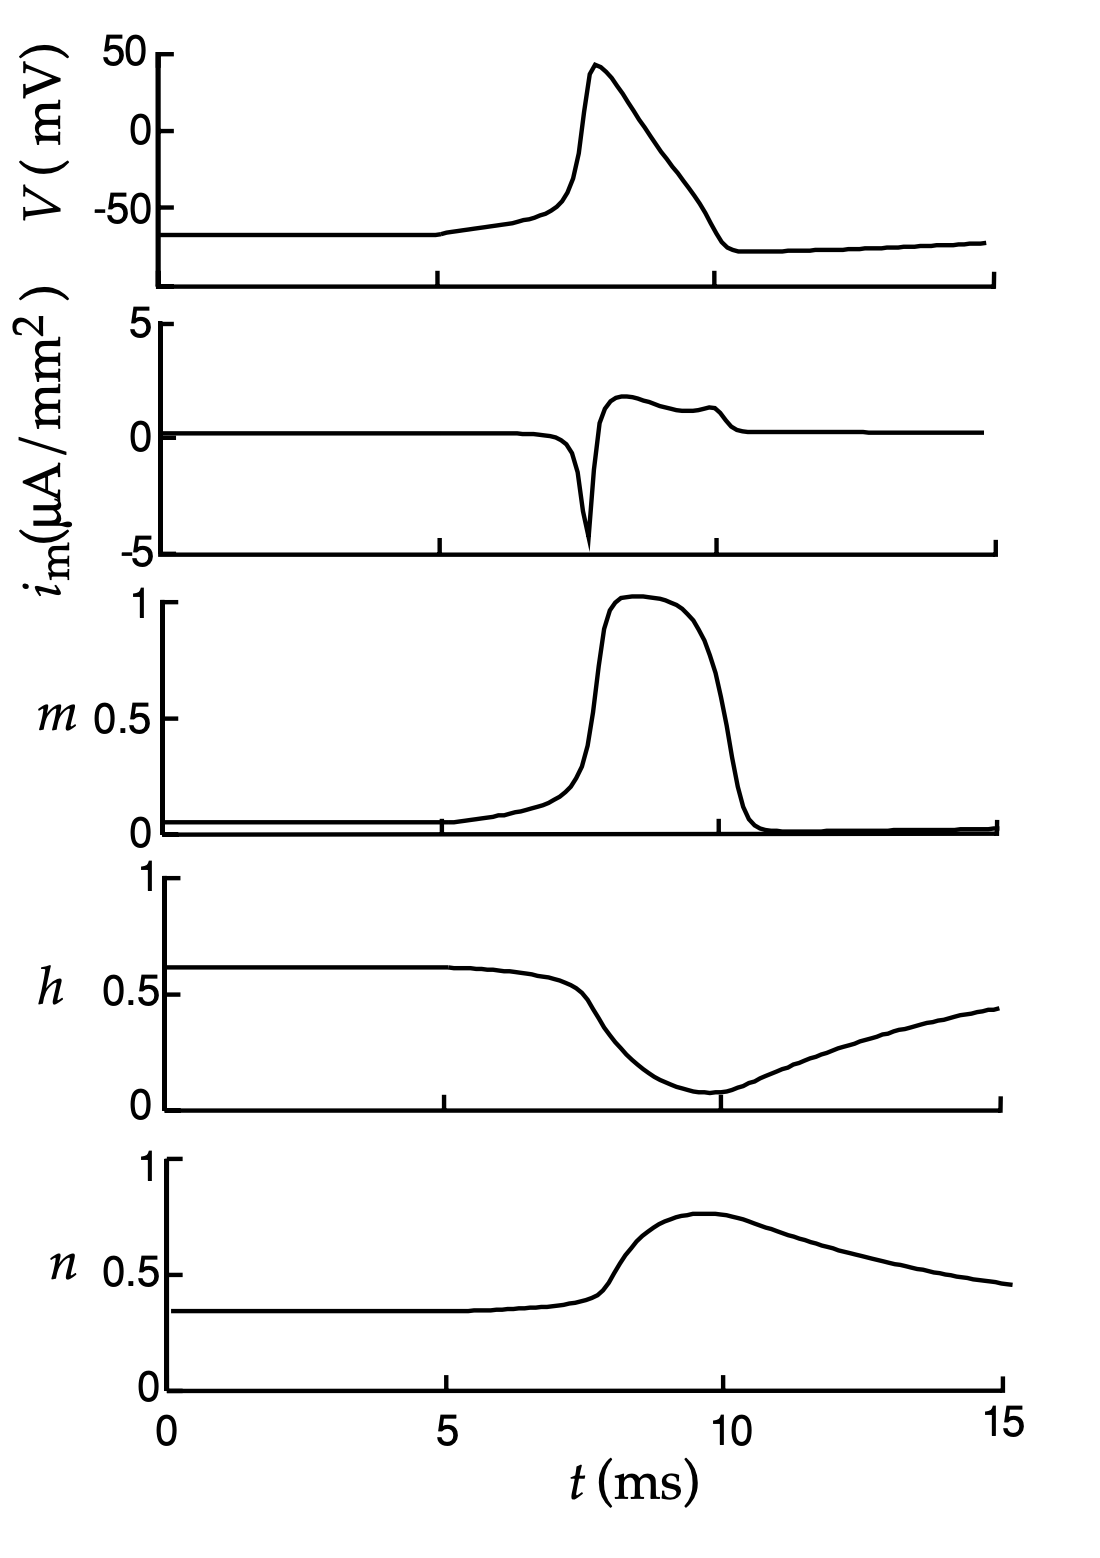
\includegraphics{H&H_Dynamics.png}\\
The dynamics of \(V\), \(m\), \(h\), and \(n\) in the Hodgkin-Huxley model during the firing of an action potential. The upper-most trace is the membrane potential, the second trace is the membrane current produced by the sum of the Hodgkin-Huxley \(K^+\) and \(Na^+\) conductances, and subsequent traces show the temporal evolution of \(m\), \(h\), and \(n\). Current injection was initiated at \(t = 5 \, \text{ms}\).}
% \begin{figure}[!ht]
% 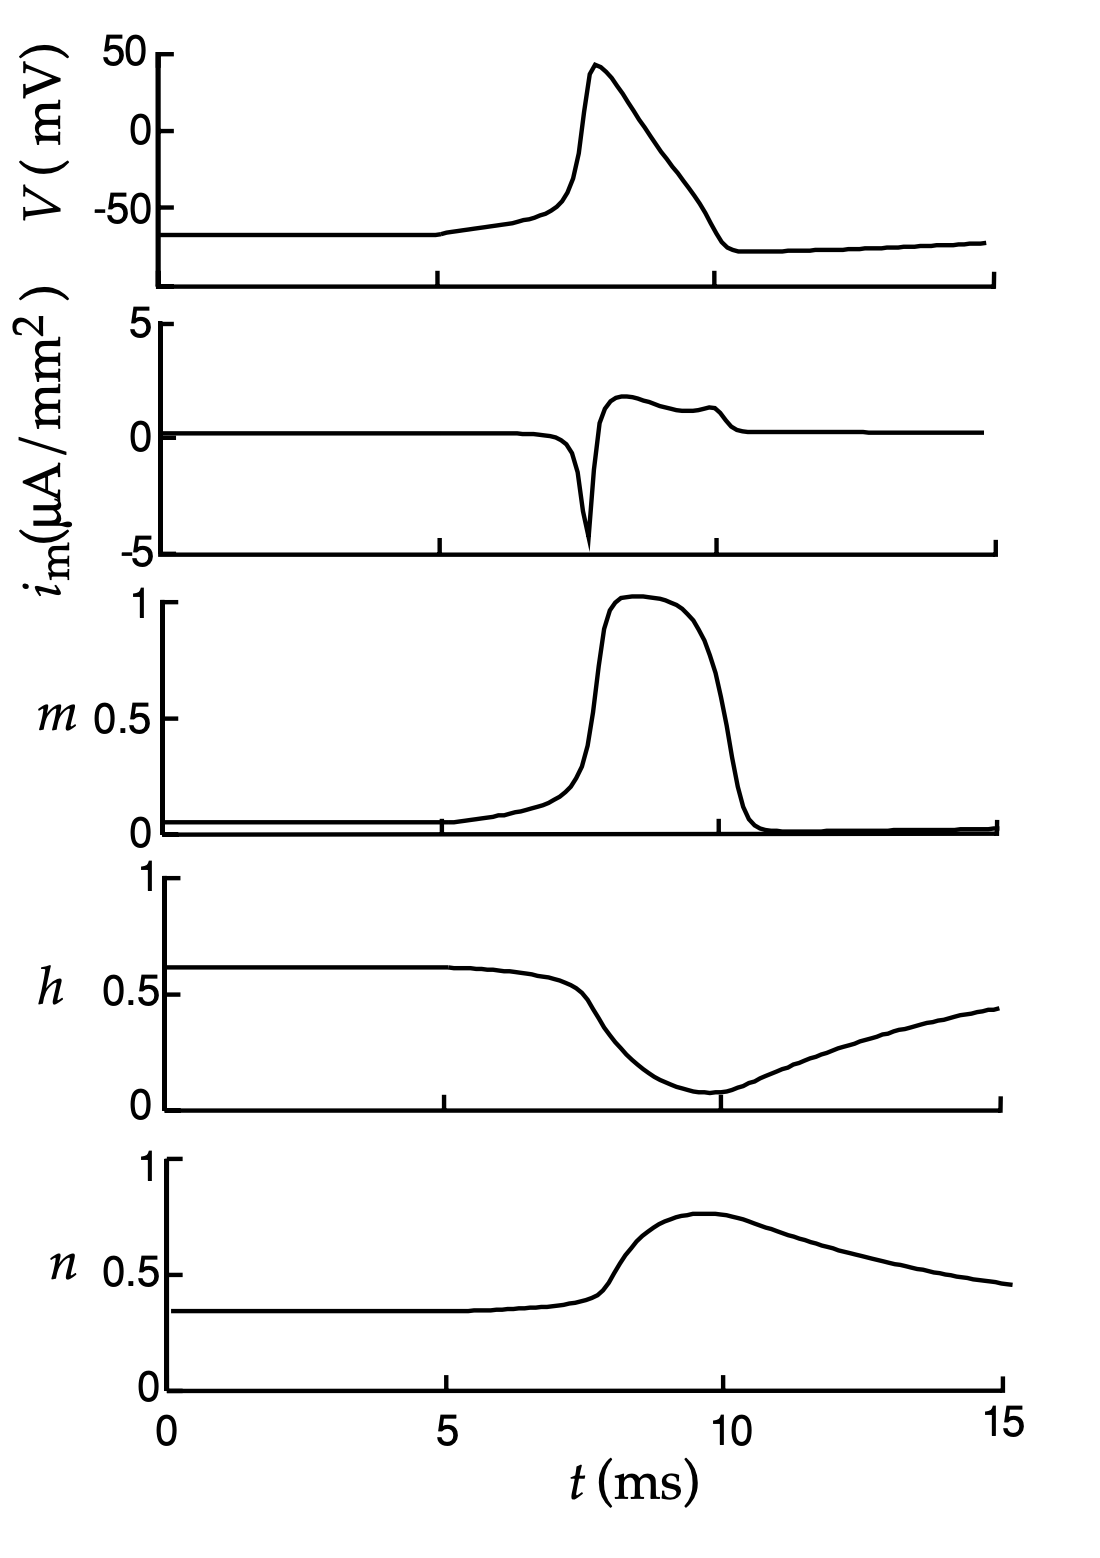
\includegraphics{H&H_Dynamics.png}
% \caption{The dynamics of \(V\), \(m\), \(h\), 
% and \(n\) in the Hodgkin-Huxley model during the 
% firing of an action potential...}
% \label{fig:HH_Dynamics}
% \end{figure}


The maximal conductances and reversal potentials used in the model are
\[
\bar{g}_L = 0.003 \, \text{mS/mm}^2, \quad \bar{g}_K = 0.36 \, \text{mS/mm}^2, \quad \bar{g}_{Na} = 1.2 \, \text{mS/mm}^2,
\]
\[
E_L = -54.387 \, \text{mV}, \quad E_K = -77 \, \text{mV}, \quad \text{and} \quad E_{Na} = 50 \, \text{mV}.
\]
The full model consists of equation 5.25 for the membrane current, and equations of the form 5.17 for the gating variables \(n\), \(m\), and \(h\). These equations can be integrated numerically, using the methods described in appendices A and B.


\textbf{Temporal evolution of dynamic variables.}\\
The initial rise of the membrane potential, prior to the action potential,
seen in the upper panel of figure below, is due to the injection of a
positive electrode current into the model starting at \(t = 5ms\).


When the current drives the membrane potential up to about -55mV, the
\( m \) variable that describes activation of the \(Na^+\) conductance suddenly jumps from 
nearly 0 to a value near 1.

Initially, the \(h\) variable, expressing the degree of inactivation of the \(Na^+\) conductance, is around 0.6. Thus, for a brief period both \(m\) and \(h\) are significantly different from 0. This causes a large influx of \(Na^+\) ions, producing the sharp downward spike of inward current shown in the second trace from the top. The inward current pulse causes the membrane potential to rise rapidly to around 50 mV (near the \(Na^+\) equilibrium potential). The rapid increase in both \(V\) and \(m\) is due to a positive feedback effect. Depolarization of the membrane potential causes \(m\) to increase, and the resulting activation of the \(Na^+\) conductance makes \(V\) increase. The rise in the membrane potential causes the \(Na^+\) conductance to inactivate by driving \(h\) toward 0. This shuts off the \(Na^+\) current. In addition, the rise in \(V\) activates the \(K^+\) conductance by driving \(n\) toward 1. This increases the \(K^+\) current, which drives the membrane potential back down to negative values. The final recovery involves the readjustment of \(m\), \(h\), and \(n\) to their initial values.



\subsection{The Hodgkin-Huxley Model: Formalization}
\marginnote{
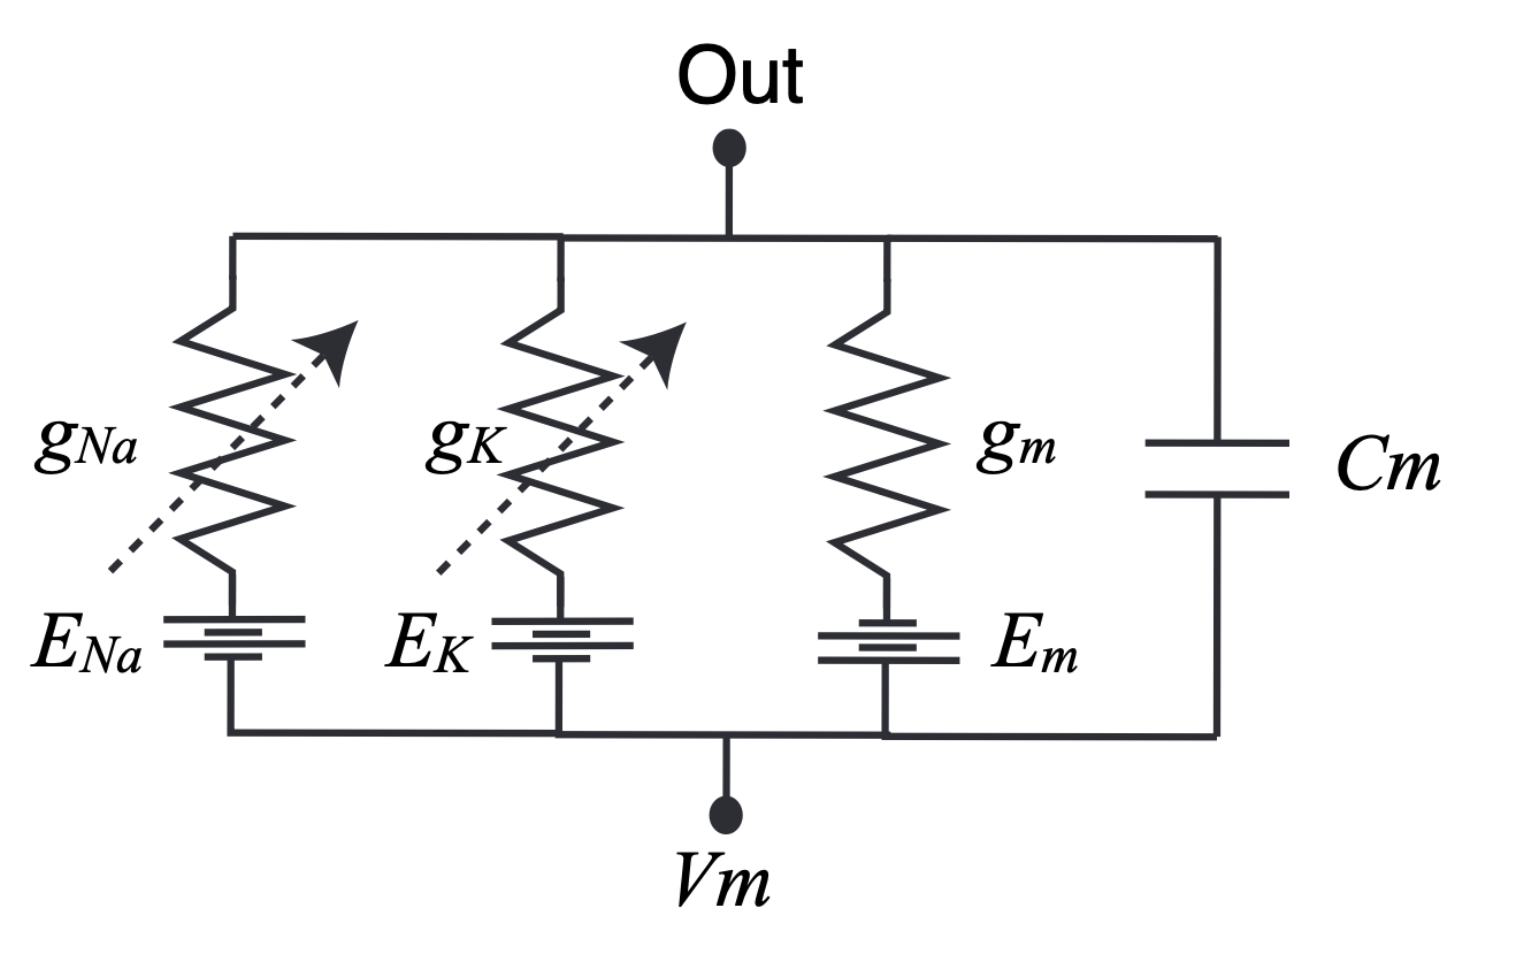
\includegraphics{H&H_Circuit.png}}
\begin{align}
  &I_c + I_m + I_{Na} + I_K = 0, \\
  &C \frac{dV_m}{dt} + g_m(V_m - E_m) + \bar{g_K}n^4(V_m - E_K) + \bar{g_{Na}}m^3h(V_m - E_{Na}) = 0,
\end{align}
where \( n,m,h \) are gating functions.

\begin{itemize}
  \item \( I_c \) is the \textbf{capacitive current}. It arices from charging or discharging the
membrane capacitor C.
  \item \( I_m \) is the \textbf{leakage (or membrane) current}.
  Given by Ohm's law, with conductance \( g_m \) and reversal potential \( E_m \).
  
  \item \( \bar{g_K}, \bar{g_{Na}} \) denotes the \textbf{maximum
  conductance} for that ion channel.
  
  \item The gating functions \( n,m,h \) give the fraction of open channels for that ion type.
  So the effective conductance would be \( \bar{g_K}n^4 \) and \( \bar{g_{Na}}m^3h \) etc.
\end{itemize}
\marginnote{Exponent on the gating function? It relects how many subunit must be open simutaneously to open the channel.}


variability neq randomness

Autocorrelation:
counts the number of coincidences spikes 

% end of main text

\makeatletter
  \renewcommand{\section}{\@startsection{section}%
    {3}{0.8em}{-3ex \@plus -1ex \@minus -.2ex}%
    {1.5ex \@plus .2ex}
    {\hspace*{-5.5em}\fcolorbox{Periwinkle}{Periwinkle}{\parbox[c][1.0ex][b]{4em}{\phantom{space}}}
    \normalfont\Large\itshape\color{blue}}}
\makeatother

\bibliography{marginnotes}
\bibliographystyle{plainnat}

\end{document}
